\documentclass[fleqn,11pt,aspectratio=1610]{beamer}

\usepackage[english]{babel}
\usepackage[utf8x]{inputenc}
\usepackage{graphicx}
\usepackage{tabularx}
\usepackage{pgfgantt} % Schedule
\usepackage{tikz}
\usepackage{tikz-uml}
\usepackage{booktabs}
\usepackage{pdflscape}
\usepackage{ifthen}
\usepackage{subfig}
\usepackage{bytefield}
\usepackage[nolist,printonlyused]{acronym}
\usetikzlibrary{positioning,fit,arrows,decorations.pathreplacing}
\usetikzlibrary{shapes,shapes.misc,positioning,circuits.ee.IEC}
\tikzstyle{system}=[shape=rounded rectangle,fill=tubsBlueLight20,text centered,draw]
\tikzstyle{sensor}=[rectangle,fill=tubsOrangeLight20,text centered,draw]
\tikzstyle{processor}=[rectangle,fill=tubsBlueLight20,text centered,draw]
\tikzstyle{connector}=[rectangle,fill=tubsGreenLight20,text centered,draw]
\tikzstyle{memory}=[rectangle,fill=tubsGreenLight20,text centered,draw]
  \tikzstyle{radio}=[rectangle,fill=tubsBlue20,text centered,draw]
\tikzstyle{bus}=[<->,color=black,draw]
\tikzstyle{buslabel}=[near end,color=black,font=\tiny,auto]
\tikzstyle{vcc}=[->,color=tubsRed,font=\tiny,draw,text=black]

\newcommand{\fitlab}{\emph{FIT IoT-LAB} }

\usetheme[%
  blue,                  % secondary color (yellow/orange/blue/green/violet)
  dark,                  % brightness (light,medium,dark)
  tocinheader,           % toc in header
  nosubsectionsinheader, % no subsections in header toc
  nexus,                 % corporate design font
  lnum,                  % NOTE: only available since tubslatex 1.01,
                         % use "Versalziffern" instead of "Mediaevalziffern"
]{tubs}

\title{Evaluating transient node failures with FIT IoT-Lab}

\subtitle{Bachelor's Thesis}

\author{Tim Schubert}

\titlegraphic[scaled]{\includegraphics{../images/ibr_logos/title_iz_corner.jpg}}

\logo{
\includegraphics{../images/ibr_logos/ibr_en.pdf}}

\begin{document}

\begin{frame}[plain]
\titlepage
\end{frame}

\section{Introduction}

\subsection{RPL}
\begin{frame}{RPL}
  \begin{columns}
    \column{.5\textwidth}
    \begin{itemize}
    \item <1-> WSN
      \begin{itemize}
      \item<2-> available energy limits network lifetime
      \item<3-> small overhead vs. quick recovery
      \end{itemize}
    \item<4-> RPL
      \begin{itemize}
      \item<5-> widespread use in applications
      \item<7-> DODAG
      \item<8-> DIS $\rightarrow$ DIO $\rightarrow$ DAO
      \item<11-> Trickle timer
      \item<12-> repair network $\rightarrow$ \textcolor{tubsRed}{increased energy usage}
      \end{itemize}
    \end{itemize}
    \column{.5\textwidth}
    \begin{figure}
      \centering
      \begin{tikzpicture}[node distance=30]
        \node[circle,fill=tubsLightGreen40] (s) {s};

        \node[circle,fill=tubsLightBlue40,below of=s,left of=s] (r11) {};
        \node[circle,fill=tubsLightBlue40,below of=s,right of=s] (r12) {};
        \node[circle,fill=tubsLightBlue40,above of=s,left of=s] (r13) {};
        \node[circle,fill=tubsLightBlue40,above of=s,right of=s] (r14) {};
        \node[circle,fill=tubsLightBlue40,below of=s] (r15) {};
        \node[circle,fill=tubsLightBlue40,above of=s] (r16) {};
        \node[circle,fill=tubsLightBlue40,left of=s] (r17) {};
        \node[circle,fill=tubsLightBlue40,right of=s] (r18) {};
        \node[circle,fill=tubsLightBlue40,left of=r11] (r21) {};
        \node[circle,fill=tubsLightBlue40,below of=r11] (r22) {};
        \node[circle,fill=tubsLightBlue40,below of=r12] (r23) {};
        \node[circle,fill=tubsLightBlue40,right of=r12] (r24) {};
        \node[circle,fill=tubsLightBlue40,left of=r13] (r25) {};
        \node[circle,fill=tubsLightBlue40,above of=r13] (r26) {};
        \node[circle,fill=tubsLightBlue40,above of=r14] (r27) {};
        \node[circle,fill=tubsLightBlue40,right of=r14] (r28) {};
        \node[circle,fill=tubsLightBlue40,above of=r16] (r30) {};
        \node[circle,fill=tubsLightBlue40,right of=r18] (r31) {};
        \node[circle,fill=tubsLightBlue40,left of=r17] (r32) {};
        \node[circle,fill=tubsLightBlue40,below of=r15] (r34) {};

        \path<8->[draw,<-] (s) -- (r16);
        \path<8->[draw,<-] (s) -- (r18);
        \path<8->[draw,<-] (s) -- (r15);
        \path<8->[draw,<-] (s) -- (r17);

        \path<9->[draw,<-] (r16) -- (r13);
        \path<9->[draw,<-] (r16) -- (r30);

        \path<9->[draw,<-] (r18) -- (r14);
        \path<9->[draw,<-] (r18) -- (r28);
        \path<9->[draw,<-] (r18) -- (r31);
        \path<9->[draw,<-] (r18) -- (r12);

        \path<9->[draw,<-] (r15) -- (r22);
        \path<9->[draw,<-] (r15) -- (r11);

        \path<9->[draw,<-] (r17) -- (r32);
        \path<9->[draw,<-] (r17) -- (r21);
        \path<9->[draw,<-] (r17) -- (r25);

        \path<10->[draw,<-] (r12) -- (r24);
        \path<10->[draw,<-] (r12) -- (r23);

        \path<10->[draw,<-] (r30) -- (r27);
        \path<10->[draw,<-] (r30) -- (r26);

        \path<10->[draw,<-] (r22) -- (r34);

      \end{tikzpicture}
    \end{figure}
  \end{columns}
\end{frame}

\subsection{Transient Node Failures}
\begin{frame}{Transient Node Failures}
  \begin{columns}
    \column{.5\textwidth}
    \begin{enumerate}
    \item <2-> hardware glitch or programming error
      \begin{itemize}
      \item \textcolor{tubsDarkGreen}{single node reset}
      \item \textcolor{tubsRed}{repeated node restarts}
      \end{itemize}
    \item <3-> detection by children (NUD / Layer 2 ACK)
      \begin{itemize}
      \item \textcolor{tubsDarkGreen}{early detection}
      \item \textcolor{tubsRed}{late detection $\rightarrow$ high packet loss}
      \end{itemize}
    \item <4-> Trickle timers reset, nodes select new parents (DIS + DIO)
      \begin{itemize}
      \item \textcolor{tubsDarkGreen}{resetting node selects parent before children}
      \item \textcolor{tubsRed}{child is selected as parent $\rightarrow$
          DAO loop $\rightarrow$ repair DAG (rank)}
      \end{itemize}
    \item <5-> advertise destinations (DAO)
      \begin{itemize}
        \item \textcolor{tubsDarkGreen}{only resetting node must be advertised}
        \item \textcolor{tubsRed}{complete sub-DODAG must be advertised}
        \end{itemize}
    \end{enumerate}

    \column{.5\textwidth}
    \begin{figure}

      \tikzstyle{root} = [draw,circle,fill=tubsLightGreen40]
      \tikzstyle{parent} = [draw,circle,fill=tubsRed!20]
      \tikzstyle{child} = [draw,circle,fill=tubsLightBlue40]

      \centering
      \begin{tikzpicture}[node distance=30]
        \node[root] (r) {s};
        \node[parent,below of=r] (p) {p};
        \node[child,below of=p,left of=p] (c1) {1};
        \node[child,below of=p,right of=p] (c2) {2};

        \path<1>[->,draw] (p) -- (r);
        \path<1-2>[->,draw] (c1) -- node {} (p);
        \path<1-2>[->,draw] (c2) -- node {} (p);

        \path<2>[-,draw,color=tubsRed,line width=5pt] (p) -- (r);
        \path<3>[-,draw,color=tubsRed,line width=5pt] (c1) --(p);
        \path<3>[-,draw,color=tubsRed,line width=5pt] (c2) -- (p);

        \path<3->[->,draw] (p)  -- (r);
        \path<4->[->,draw] (c1) -- (p);
        \path<4->[->,draw] (c2) -- (p);
      \end{tikzpicture}

    \end{figure}

    \centering
    \visible<6->{\textcolor{tubsDarkBlue}{we want fewer messages and quick recovery}}
  \end{columns}

\end{frame}

\subsection{Persistent Routing Information}
\begin{frame}{Persistent Routing Information}
  \begin{columns}
    \column{.6\textwidth}
    \begin{itemize}
      \item<1-> implemented and evaluated using simulations by Silas Müller
      \item<2-> ported to \fitlab hardware
      \item<3-> store latest updates to RPL state (DIO) in persistent memory
      \item<4-> restore state / replay changes after restart
      \item<5-> \textcolor{tubsDarkGreen}{$\rightarrow$ quicker recovery with
          less (radio) overhead}
      \item<6-> extension: use clocks and UIDs to validate state
    \end{itemize}
    \column{.4\textwidth}
    \begin{figure}
    \begin{bytefield}{20}
      \wordbox[tlr]{1}{\small{Magic Byte}} \\
      \wordbox[tlr]{1}{\small{Constant Parameters}} \\
      \wordbox[tlr]{1}{\small{Neighbor Addresses \ldots}} \\
      \wordbox[tlr]{1}{\small{Neighbor Count}} \\
      \wordbox[tlr]{1}{\small{DIO Interval}} \\
      \wordbox[tlr]{1}{\small{Neighbor Updates (DIO) \ldots}}
    \end{bytefield}
    \end{figure}
  \end{columns}
\end{frame}

\subsection{FIT IoT-LAB}

\begin{frame}{FIT IoT-LAB}
  \begin{columns}
    \column{.6\textwidth}
    \begin{itemize}
    \item<1-> very large scale (> 2000 nodes) automated testbed for WSN applications by \emph{Inria}
    \item<2-> federates with other testlabs (\emph{OneLab})
    \item<3-> API
      \begin{itemize}
      \item create experiments
      \item program nodes
      \item access results
      \end{itemize}
    \item<4-> Site Server
      \begin{itemize}
      \item collects and stores logs
      \item gateway to testlab nodes
      \end{itemize}
    \end{itemize}

    \column{.4\textwidth}
    \centering
    \includegraphics<1->[height=.4\textheight]{../images/lille_8032.png}
    \visible<3->{%
    \begin{figure}
      \centering
      \usetikzlibrary{fit}
      \scalebox{.5}{%
        \begin{tikzpicture}
          \node (U) at (0,0) [shape=circle,draw,fill=tubsLightGreen20] {User};
          \node (A) at (3,0) [fill=tubsLightOrange20,shape=rounded rectangle,draw] {API};
          \node (S) at (6,0) [fill=tubsLightOrange20,shape=rectangle,draw] {Site Server};
          \path (U) edge [arrows=<->,auto,swap] node {REST} (A);
          \path (U) edge [arrows=<->,bend left] node [auto,swap] {SSH} (S);
          \path (A) edge [arrows=<->] (S);
          \node (n1) at (8.5,-1) [fill=tubsLightBlue20,shape=ellipse,draw] {Node};
          \node (n2) at (8.5,0) [fill=tubsLightBlue20,shape=ellipse,draw] {Node};
          \node (n3) at (8.5,1) [fill=tubsLightBlue20,shape=ellipse,draw] {Node};
          \foreach \n in {n1,n2,n3} \path (\n) edge [arrows=<->,auto,swap] (S);
          \path (A) edge [arrows=<->] (S);
          \begin{pgfonlayer}{background}
            \node [label=above:Intranet,fill opacity=0.2,shape=rounded rectangle,fill=tubsLightViolet80,fit=(n1)(n2)(n3)(S)] {};
            \node [label=below left:Internet,fill opacity=0.2,shape=rounded rectangle,fill=tubsLightBlue80,fit=(U)(A)(S)] {};
          \end{pgfonlayer}
        \end{tikzpicture}
      }
    \end{figure}
    }
  \end{columns}
\end{frame}

\begin{frame}{M3 Open Sensor Node}

  \begin{columns}
    \column{.6\textwidth}
    \begin{itemize}
    \item <1-> ON
      \begin{itemize}
      \item CPU: STM32F103REY (32-bit, ARM Cortex-M3)
      \item Memory: N25Q128 (128MByte, external NOR-Flash)
      \item Radio: AT86RF231 (2.4 GHz, IEEE 802.15.4 support)
      \end{itemize}
    \item <2-> CN
      \begin{itemize}
      \item accesses sensors
      \item controls power supply
      \item flashes the node
      \end{itemize}
    \item <3-> GW
      \begin{itemize}
      \item forwards serial output to TCP socket
      \item provides remote debugger
      \end{itemize}
    \end{itemize}

    \column{.4\textwidth}
  \centering
  \resizebox{!}{.6\textheight}{%
  \begin{tikzpicture}
    \node[processor] (cpu)[minimum width=50,minimum height=50] {M3}; %STM32F103RKEY

    \node[memory] (flash) [below of=cpu,below=0.5] {Flash}; %N25Q128A
    \draw[bus,transform canvas={xshift=-10}] (flash) edge node[buslabel] {GPIO} (cpu);
    \draw[bus,transform canvas={xshift=10}] (flash) edge node[buslabel] {SPI} (cpu);

    \node[radio] (wireless) [right of=cpu,above of=cpu,right=0.4] {Radio}; %AT86RF231
    \path[bus] (wireless.240) |- node[buslabel,above] {GPIO} (cpu.10);
    \path[bus] (wireless) |- node[buslabel] {SPI} (cpu);

    \node[system] (usbb) [above of=cpu,above=1] {USB Bridge};
    \path[bus] (usbb) edge node[buslabel] {JTAG} (cpu);
    \path[bus,transform canvas={xshift= 20}] (usbb) edge node[buslabel] {UART} (cpu);

    \node[connector] (oc) [above of=usbb,above=1,minimum width=100] {Open Node Connector};
    \path[bus] (usbb) edge node[buslabel]{USB} (oc) ;
    \path[bus] (oc.190) |- node[buslabel]{GPIO} (cpu.160) ;

    \node[connector] (usb) [right of=oc,below of=oc,right=0.5] {USB};
    \path[bus] (oc) |- (usb);

    \node[processor] (pm) [below of=usb] {Power};

    \node[sensor] (light)   [minimum width=80,below left of=oc,left=1.5] {Light Sensor}; %ISL29020
    \node[sensor] (pressure)[minimum width=80,below of=light] {Pressure Sensor}; %LPS331AP
    \node[sensor] (gyro)    [minimum width=80,below of=pressure] {Gyroscope}; %L3G4200D
    \node[sensor] (magneto) [minimum width=80,below of=gyro] {Magnetometer}; %LSM303DLHC

    \path[bus] (oc.188) |- (light);
    \path[bus] (oc.188) |- (gyro);
    \path[bus] (oc.188) |- (magneto);
    \path[bus] (oc.188) |- (pressure);
    \path[bus] (oc.188) |- node[buslabel,below] {I2C} (cpu.190);
    \path[bus] (gyro)   -| node[buslabel,below] {GPIO} (cpu.120);
    \path[bus] (magneto.10)-| (cpu.120);

    \path[vcc] (pm.210) |- node[below] {+3.3 V} (usbb);
    \path[vcc,orange,text=black] (pm) -- node[auto] {+3.3 V mon.} (wireless);
    \path[vcc] (usb) -- node[left] {+5} (pm);
    \path[vcc] (oc.340) |- node[near start,auto] {+3.3} (pm.165);
    \path[vcc,orange,text=black] (oc.330) |- node[near start,left] {+5} (pm.175);

    \path[vcc,orange,text=black] (pm) |- (1,1.8) -| (cpu.70);
    \path[vcc,orange,text=black] (pm) |- (1,1.8) -- (0.5,1.8);
    \node[rounded rectangle,right of=pm,right=0.1] (gnd) {GND};
    \path[vcc,<->] (pm) -- (gnd);

  \end{tikzpicture}
  }
  \visible<2->{%
      \centering
      \resizebox{!}{.2\textheight}{%
      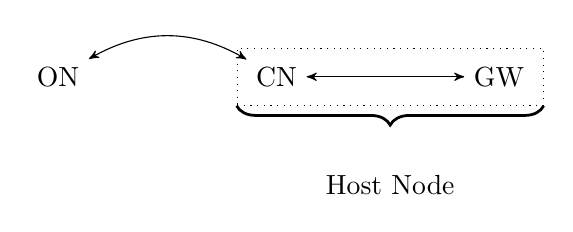
\begin{tikzpicture}[node/.style={circle,draw}]
        \begin{scope}[node distance=2cm]
          \node (a) {ON};
          \node (b) [right=of a] {CN};
          \node (c) [right=of b] {GW};
        \end{scope}

        \begin{scope}[<->,>=stealth',auto]
          \path (a) edge[bend left] (b)
          (b) edge (c);
        \end{scope}

        \node[draw,dotted,fit=(b)(c)](group){};
        \draw[line width=1pt,black,decorate,decoration={amplitude=7pt,brace,mirror}]
        (group.south west) -- (group.south east);
        \node[below=of group,anchor=center]{Host Node};
      \end{tikzpicture}
      }
      }

  \end{columns}
\end{frame}

\section{Measurement Setup}

\begin{frame}{Measurement Setup}
  \begin{columns}
    \column{.3\textwidth}
  \begin{enumerate}
  \item <1-> setup experiment using API
  \item <2-> collect results from shared server
  \item <3-> parse, aggregate and save results into database
  \item <4-> analyze and visualize results
  \end{enumerate}

  \column{.7\textwidth}
\begin{figure}
  \centering

  \scalebox{.4}{%
  \begin{tikzpicture}
    \tikzumlset{fill component=tubsLightBlue20, fill port=tubsLightBlue40}

    \begin{umlcomponent}[x=-0.5,y=15,fill=white]{Testlab Node}
    \end{umlcomponent}
    \begin{umlcomponent}[x=3.5,y=15,fill=white]{Testlab Node}
    \end{umlcomponent}
    \begin{umlcomponent}[x=7.5,y=15,fill=white]{Testlab Node}
    \end{umlcomponent}

    \begin{umlcomponent}[x=-1,y=14,fill=white]{Testlab Node}
    \end{umlcomponent}
    \begin{umlcomponent}[x=3,y=14,fill=white]{Testlab Node}
    \end{umlcomponent}
    \begin{umlcomponent}[x=7,y=14,fill=white]{Testlab Node}
    \end{umlcomponent}

    \begin{umlcomponent}[y=1]{Testlab Node}
      \begin{umlcomponent}{Open Node}
        \umlbasiccomponent{UDP Sink / Source}
        \umlbasiccomponent[y=3]{Logger}
        \umlbasiccomponent[y=6]{Powertrace}
      \end{umlcomponent}

      \begin{umlcomponent}[x=6]{Host Node}
        \umlbasiccomponent{Consumption}
        \umlbasiccomponent[y=2.5]{RSSI}
        \umlbasiccomponent[y=5]{Event Log}
        \umlbasiccomponent[y=7.5]{Sniffer}
        \umlbasiccomponent[y=10]{Forwarded Serial}
      \end{umlcomponent}
    \end{umlcomponent}

    \begin{umlcomponent}[y=1,x=14.5]{Shared Server}
      \umlbasiccomponent[y=2.5]{Log files}
      \umlbasiccomponent[y=5]{Sniffer Aggregator}
      \umlbasiccomponent[y=7.5]{Serial Aggregator}
    \end{umlcomponent}

    \begin{umlcomponent}[y=1,x=20,fill=tubsLightGreen20]{Local Computer}
      \umlbasiccomponent[y=12]{Orchestration}
      \umlbasiccomponent[y=8]{Database}
      \umlbasiccomponent[y=4]{Analysis}
      \begin{umlcomponent}[y=0]{Presentation}
        \umlactor[scale=0.5]{User}
      \end{umlcomponent}

      \umlassemblyconnector[interface=Parser]{Database-north-port}{Orchestration-south-port}
      \umlassemblyconnector[interface=SQL]{Analysis-north-port}{Database-south-port}
      \umlassemblyconnector[interface=Python]{Presentation-north-port}{Analysis-south-port}

    \end{umlcomponent}

    \umlbasiccomponent[x=14.5,y=14,fill=tubsLightBlue20]{API Server}
    \umlassemblyconnector[interface=REST,with port]{Orchestration-west-port}{API Server}
    \umlassemblyconnector[interface=SSH,with port]{API Server-south-port}{Shared Server-north-port}

    \umlassemblyconnector[interface=SSH,with port]{Orchestration}{Shared Server}
    \umlassemblyconnector[interface=ON Con,with port]{Host Node}{Open Node}
    %\umlHVHassemblyconnector[interface=Configuration,with port]{API}{Host Node}
    \umlHVHassemblyconnector[with port,arm2=+2cm]{Log files}{Consumption}
    \umlassemblyconnector[interface=Log Collection,with port]{Log files}{RSSI}
    \umlHVHassemblyconnector[with port,arm2=+2cm]{Log files}{Event Log}
    \umlassemblyconnector[interface=TCP,with port]{Serial Aggregator}{Forwarded Serial}
    \umlassemblyconnector[interface=TCP,with port]{Sniffer Aggregator}{Sniffer}
  \end{tikzpicture}
  }
\end{figure}
\end{columns}
\end{frame}

\section{Evaluation}

\subsection{Configurations}

\begin{frame}{Configurations}
  \begin{columns}
    \column{.6\textwidth}
    \begin{itemize}
    \item<1-> 44 nodes, 50 runs
    \item<2-> phases
      \begin{itemize}
      \item N - default \emph{Contiki}-RPL
      \item H - \emph{Contiki}-RPL with restoring of persistent state
      \item HS - H + validation
      \item *R - single node reset at random time
      \item 60 s guard interval at beginning and end of phase
      \end{itemize}
    \item<3-> compare different phases
      \begin{itemize}
      \item same experiment with different firmware settings
      \item run different firmwares in close succession
      \item reconstruct beginning / end of each phase from log files
      \end{itemize}
    \end{itemize}
    \column{.4\textwidth}
    \begin{table}[h]
      \centering
      \footnotesize
      \begin{tabular}{r c c c}
        \toprule
        Test run & Hardened & Validity & Resets \\
        \midrule
        N   &   &   &   \\
        R   &   &   & X \\
        H   & X &   &   \\
        HR  & X &   & X \\
        HS  & X & X &   \\
        HSR & X & X & X \\
      \end{tabular}
    \end{table}
  \end{columns}
\end{frame}

\begin{frame}{Route stability}
  \begin{figure}
    \centering
    \includegraphics[height=\textheight]{../images/routes.pdf}
  \end{figure}
\end{frame}

\subsection{Topology}
\begin{frame}{Route changes}
  \begin{columns}
    \column{.5\textwidth}
    \begin{itemize}
    \item<1-> changes increase \textcolor{tubsRed}{energy consumption}
    \item<2-> restoring previous state causes additional (unwanted) changes
    \item<3-> still (!) H and HS reduce number of changes enough to get below R
    \item<4-> \textcolor{tubsDarkGreen}{$\rightarrow$ persistence reduces effect
        of reset on DAG}
    \end{itemize}
    \column{.5\textwidth}
    \begin{figure}
    \centering
    \includegraphics[width=\textwidth]{../images/stability.pdf}
  \end{figure}
  \end{columns}
\end{frame}

\begin{frame}{Convergence Time}
  \begin{columns}
    \column{.5\textwidth}
    \begin{itemize}
      \item<1-> time until last node has acquired a default route
      \item<2-> large error due to restoring state
      \item<3-> validation in HS saves some time
      \item<4-> setup process is similar to repair process (\textcolor{tubsRed}{recovery time})
    \end{itemize}
    \column{.5\textwidth}
    \begin{figure}
      \centering
      \includegraphics[width=\textwidth]{../images/convergence.pdf}
    \end{figure}
  \end{columns}
\end{frame}

\subsection{Network Performance}

\begin{frame}{End-to-End}
  \begin{columns}

    \column{.5\textwidth}
    \begin{itemize}
       \item<1-> single trip from source to sink (root)
       \item<2-> delay: no significant difference
       \item<3-> loss
         \begin{itemize}
         \item<4-> HS[R] takes longer to recover
         \item<5-> HS[R] less affected by resets
         \end{itemize}
    \end{itemize}

    \column{.5\textwidth}
    \begin{figure}
      \includegraphics<1>[width=\textwidth]{../images/performance-delay.pdf}
      \includegraphics<3->[width=\textwidth]{../images/performance-loss.pdf}
    \end{figure}
  \end{columns}
\end{frame}

\begin{frame}{Message Overhead}
  \begin{columns}
    \column{.5\textwidth}
    \begin{itemize}
    \item<1-> large part of \textcolor{tubsRed}{energy consumption}
    \item<2-> default implementation creates the fewest messages
      \begin{itemize}
      \item old state was restored, then invalidated
      \end{itemize}
    \item<3-> HS most messages and largest error
      \begin{itemize}
      \item validation of restored state
      \end{itemize}
    \item<5-> \textcolor{tubsDarkGreen}{restore state $\rightarrow$ reduces
        overhead from reset}
    \end{itemize}
    
    \column{.5\textwidth}
    \begin{figure}
      \centering
      \includegraphics[width=\textwidth]{../images/performance-overhead.pdf}
    \end{figure}
    \end{columns}
\end{frame}

\subsection{Energy Consumption}

\begin{frame}{Energy Consumption}
  \begin{columns}
    \column{.5\textwidth}
    \begin{itemize}
    \item<1-> N, H, HS
      \begin{itemize}
      \item default implementation consumes less energy (old state is restored)
      \end{itemize}
    \item<2-> *R
      \begin{itemize}
      \item small improvement over default implementation
      \item validation consumes more energy than it saves
      \end{itemize}
    \item<3-> measurement error between phases
      \begin{itemize}
      \item see measurement series for individual nodes
      \item unrelated to single node restart
      \item $\rightarrow$ issue with HN?
      \end{itemize}
    \end{itemize}
    \column{.5\textwidth}
  \begin{figure}
    \centering
    \includegraphics[width=\textwidth]{../images/consumption-phases.pdf}
  \end{figure}
  \end{columns}
\end{frame}

\section{Demo}

\begin{frame}{Demo}

\end{frame}

\section{Conclusion}

\begin{frame}{Conclusion}
  \begin{itemize}
    \item<1-> analyze effect of transient node failures
    \item<2-> automated deployment, collection, analysis, visualisation
    \item<3-> ported hardened RPL version to \fitlab hardware
    \item<4-> unwanted repairs after intentional restarts
      \begin{itemize}
      \item how to tell node that restart was intentional?
      \end{itemize}
    \item<5-> persistence improves
      \begin{itemize}
      \item number of changes
      \item consumption
      \item overhead
      \end{itemize}
    \item<6-> additional validation
      \begin{itemize}
      \item no practical advantage
      \item consumes more energy
      \item slower recovery
      \end{itemize}
    \end{itemize}
\end{frame}

%\bibliographystyle{abbrv}
%\bibliography{../bibliography}

\begin{frame}{Consumption}
  \begin{table}
    \centering
    \begin{tabular}{lp{140pt}}
      \toprule
      Component & Current Consumption (3.3 V) \\
      \midrule
      CPU & 70 mA \\
      Radio & SLEEP 20 $\mu$A \newline
              OFF 0.4 mA \newline
              RX 10.3 mA \newline
              TX 10 mA\\
      Flash & 20 mA 
    \end{tabular}
    \label{tab:consum}
  \end{table}
\end{frame}

\tikzstyle{cnode}=[circle,fill=tubsLightOrange100,text centered,font=\tiny,fill
opacity=0.5,draw opacity=0.5,text opacity=1.0]
\tikzstyle{snode}=[circle,fill=tubsGray20,text centered,font=\tiny,fill
opacity=0.2,draw opacity=0.2,text opacity=1.0]
\tikzstyle{pnode}=[circle split,draw,text centered,fill=tubsLightOrange20,draw opacity=0.1,text opacity=1.0,fill opacity=0.1,font=\tiny]

%TODO latex number vs strings wtf

\newcommand{\fitnode}[3]{%
  \ifthenelse
  {#3 = 47 \OR #3 = 49 \OR #3 = 51 \OR #3 = 53 \OR #3 = 57 \OR #3 = 59 \OR #3 = 83 \OR #3 = 85 \OR #3 = 87 \OR #3 = 89 \OR #3 = 91 \OR #3 = 93 \OR #3 = 95 \OR #3 = 123 \OR #3 = 127 \OR #3 = 131 \OR #3 = 133 \OR #3 = 151 \OR #3 = 153 \OR #3 = 155 \OR #3 = 157 \OR #3 = 159 \OR #3 = 161 \OR #3 = 192 \OR #3 = 194 \OR #3 = 196 \OR #3 = 198 \OR #3 = 200 \OR #3 = 202 \OR #3 = 204 \OR #3 = 218 \OR #3 = 220 \OR #3 = 222 \OR #3 = 224 \OR #3 = 226 \OR #3 = 228 \OR #3 = 230 \OR #3 = 244 \OR #3 = 246 \OR #3 = 248 \OR #3 = 250 \OR #3 = 252 \OR #3 = 254 \OR #3 = 256}%\isin{47}{ \OR #3 = 47 \OR #3 = 49 \OR #3 = 51 \OR #3 = 53 \OR #3 = 57 \OR #3 = 59 \OR #3 = 83 \OR #3 = 85 \OR #3 = 87 \OR #3 = 89 \OR #3 = 91 \OR #3 = 93 \OR #3 = 95 \OR #3 = 123 \OR #3 = 127 \OR #3 = 131 \OR #3 = 133 \OR #3 = 151 \OR #3 = 153 \OR #3 = 155 \OR #3 = 157 \OR #3 = 159 \OR #3 = 161 \OR #3 = 192 \OR #3 = 194 \OR #3 = 196 \OR #3 = 198 \OR #3 = 200 \OR #3 = 202 \OR #3 = 204 \OR #3 = 218 \OR #3 = 220 \OR #3 = 222 \OR #3 = 224 \OR #3 = 226 \OR #3 = 228 \OR #3 = 230 \OR #3 = 244 \OR #3 = 246 \OR #3 = 248 \OR #3 = 250 \OR #3 = 252 \OR #3 = 254 \OR #3 = 256}}
  {\node at (#1,#2) [cnode] {#3};}
  {\node at (#1,#2) [snode] {#3};}
}
\begin{frame}{Topology}

\begin{figure}
  \centering

  \usetikzlibrary{shapes}

  \resizebox{!}{.9\textheight}{%
  \begin{tikzpicture}
    \draw [black!20] (-0.3,13) -- (7.5,13) -- (7.5,4.8) -- (8.7,4.8) -- (8.7,0.8) -- (4.2,0.8) -- (4.2,-0.6) -- (-0.3,-0.6) -- cycle;
    \draw [tubsBlack!20] (8.7,13) -- (13.2,13) -- (13.2,-0.6) -- (8.7,-0.6) -- cycle;
    \fill [tubsLightGreen] (4.7,12.4) rectangle (5.3,12.9);
    \fill [tubsBlack!20] (-0.3,9.2) rectangle (-0.2,11.9);
    \fill [tubsBlack!20] (-0.3,0.2) rectangle (-0.2,2.6);
    \fill [tubsBlack!20] (0,13) rectangle (2.2,13.1);
    \draw [tubsBlack!20] (-0.4,3.95) rectangle (-0.3,4.1);
    \draw [tubsBlack!20] (-0.4,7.95) rectangle (-0.3,8.10);
    \draw [tubsBlack!20] (4.05,3.75) rectangle (4.2,3.9);
    \draw [tubsBlack!20] (4.05,8.05) rectangle (4.2,8.2);
    \draw [tubsBlack!20] (7.40,8.05) rectangle (7.55,8.2);
    \draw [tubsBlack!20] (8.65,3.75) rectangle (8.80,3.9);
    \foreach \x in {0,1,...,4} {
      \foreach \y in {0,1,...,12} {
        \pgfmathparse{int(29+\x*18+(12-\y))}
        \edef\p{\pgfmathresult}
        \fitnode{\x}{\y}{\p}
      }
    }
    \foreach \x in {0,1,...,2} {
      \foreach \y in {1,2,...,12} {
        \pgfmathparse{int(123+\x*14+(12-\y))}
        \edef\p{\pgfmathresult}
        \fitnode{\x+5}{\y}{\p}
      }
    }
    \foreach \y in {1,2,...,7} {
      \pgfmathparse{int(190-\y)}
      \edef\p{\pgfmathresult}
      \fitnode{8}{\y}{\p}
    }
    \foreach \y in {9,10,...,12} {
      \pgfmathparse{int(191-\y)}
      \edef\p{\pgfmathresult}
      \fitnode{8}{\y}{\p}
    }
    \foreach \x in {0,1,...,4} {
      \foreach \y in {0,1,...,12} {
        \pgfmathparse{int(256-(4-\x)*13-\y)}
        \edef\p{\pgfmathresult}
        \fitnode{\x+9}{\y}{\p}
      }
    }
    \foreach \y in {0,2,...,24} {
      \pgfmathparse{int(25-\y)}
      \edef\p{\pgfmathresult}
      \pgfmathparse{int(\p+1)}
      \edef\q{\pgfmathresult}
      \node at (-0.3,\y/2) [pnode] {\p \nodepart{lower} \q};
    }
    \node at (0,13) [pnode] {27 \nodepart{lower} 28};
    \node at (1,13) [pnode] {45 \nodepart{lower} 46};
    \node at (2,13) [pnode] {63 \nodepart{lower} 64};
    \node at (3,13) [pnode] {81 \nodepart{lower} 82};
    \node at (4,13) [pnode] {99 \nodepart{lower} 100};
    \node at (0,-1) [pnode] {42,43 \nodepart{lower} 44};
    \node at (1,-1) [pnode] {60,61 \nodepart{lower} 62};
    \node at (2,-1) [pnode] {78,79 \nodepart{lower} 80};
    \node at (3,-1) [pnode] {96,97 \nodepart{lower} 98};
    \node at (4,-1) [pnode] {114,115 \nodepart{lower} 116};
    \node at (4.3,0.8) [pnode] {\nodepart{lower} 121,122};
    \node at (5,0.8) [pnode] {\nodepart{lower} 135,136};
    \node at (6,0.8) [pnode] {\nodepart{lower} 149,150};
    \node at (7,0.8) [pnode] {\nodepart{lower} 163,164};
    \node at (8,0.8) [pnode] {\nodepart{lower} 190,191};
    \foreach \y in {0,2,4,6,8} {
      \pgfmathparse{int(177-\y)}
      \edef\p{\pgfmathresult}
      \pgfmathparse{int(\p+1)}
      \edef\q{\pgfmathresult}
      \node at (7.5,\y/2+5) [pnode] {\p \nodepart{lower} \q};
    }
    \foreach \y in {12,14} {
      \pgfmathparse{int(179-\y)}
      \edef\p{\pgfmathresult}
      \pgfmathparse{int(\p+1)}
      \edef\q{\pgfmathresult}
      \node at (7.5,\y/2+5) [pnode] {\p \nodepart{lower} \q};
    }
    \node at (4.2,3.9) [pnode] {\nodepart{lower} 119,120};
    \node at (4.2,8.1) [pnode] {117,118};
  \end{tikzpicture}
  }
\end{figure}
  \end{frame}

\begin{frame}{Measured Variables}
\begin{table}[h]
  \centering
  \begin{tabular}{ll}
    \toprule
    Variable & Source \\
    \midrule
    Network latency & PCAP, serial output \\
    Delivery ratio & PCAP, serial output \\
    Message overhead & PCAP, serial output \\
    Number of DIO, DAO & PCAP, serial output \\
    DODAG state & serial output \\
    Routing table & serial output \\
    Node reset times & HN event log \\
    RSSI & HN radio receiver \\
    Energy consumption & HN power monitor \\
  \end{tabular}
\end{table}
\end{frame}

\begin{frame}{Consumption by Position}
  \begin{figure}
    \centering
    \includegraphics[height=.9\textheight]{../images/consumption-nodes.pdf}
  \end{figure}
\end{frame}

\begin{frame}{Consumption of (node 200, exp-id 107077)}
  \centering
  \includegraphics[height=\textheight]{../images/200-consum.png}
\end{frame}

\begin{frame}{DODAG example}
  \centering
  \includegraphics[width=\textwidth]{../images/dag.pdf}
\end{frame}

\end{document}
